% !TEX TS-program = pdflatex
% !TEX encoding = UTF-8 Unicode

% This is a simple template for a LaTeX document using the "article" class.
% See "book", "report", "letter" for other types of document.

\documentclass[11pt]{article} % use larger type; default would be 10pt

\usepackage[utf8]{inputenc} % set input encoding (not needed with XeLaTeX)
\usepackage[spanish]{babel}

%%% Examples of Article customizations
% These packages are optional, depending whether you want the features they provide.
% See the LaTeX Companion or other references for full information.

%%% PAGE DIMENSIONS
\usepackage{geometry} % to change the page dimensions
\geometry{a4paper} % or letterpaper (US) or a5paper or....
% \geometry{margin=2in} % for example, change the margins to 2 inches all round
% \geometry{landscape} % set up the page for landscape
%   read geometry.pdf for detailed page layout information

\usepackage{graphicx} % support the \includegraphics command and options
\usepackage{caption}
\usepackage{subcaption}
% \usepackage[parfill]{parskip} % Activate to begin paragraphs with an empty line rather than an indent

%%% PACKAGES
\usepackage{booktabs} % for much better looking tables
\usepackage{array} % for better arrays (eg matrices) in maths
\usepackage{paralist} % very flexible & customisable lists (eg. enumerate/itemize, etc.)
\usepackage{verbatim} % adds environment for commenting out blocks of text & for better verbatim
\usepackage{subfig} % make it possible to include more than one captioned figure/table in a single float
\usepackage{mwe}
\usepackage{url}
% These packages are all incorporated in the memoir class to one degree or another...

%%% HEADERS & FOOTERS
\usepackage{fancyhdr} % This should be set AFTER setting up the page geometry
\pagestyle{fancy} % options: empty , plain , fancy
\renewcommand{\headrulewidth}{0pt} % customise the layout...
\lhead{}\chead{}\rhead{}
\lfoot{}\cfoot{\thepage}\rfoot{}

%%% SECTION TITLE APPEARANCE
\usepackage{sectsty}
\allsectionsfont{\sffamily\mdseries\upshape} % (See the fntguide.pdf for font help)
% (This matches ConTeXt defaults)

%%% ToC (table of contents) APPEARANCE
\usepackage[nottoc,notlof,notlot]{tocbibind} % Put the bibliography in the ToC
\usepackage[titles,subfigure]{tocloft} % Alter the style of the Table of Contents
\renewcommand{\cftsecfont}{\rmfamily\mdseries\upshape}
\renewcommand{\cftsecpagefont}{\rmfamily\mdseries\upshape} % No bold!

%%% END Article customizations

%%% The "real" document content comes below...

\title{CLP Lab 0 Report}
\author{Albert Aparicio Isarn\\
	\url{albert.aparicio.isarn@alu-etsetb.upc.edu}
	\and 
	Héctor Esteban\\
	\url{hect.esteban@gmail.com}}
\date{} % Activate to display a given date or no date (if empty),
         % otherwise the current date is printed 

\begin{document}
\maketitle

\section{Test de gaussianidad de distribuciones sintéticas}

Como se puede ver en la figura \ref{fig:22:distributions}, los gráficos de las distribuciones \emph{Rayleigh}, \emph{Laplaciana} y \emph{Uniforme} son visiblemente distintos a los de la distribución. 

Estas diferencias se ven más claramente en los \emph{NormPlot} y los gráficos de \emph{Skewness} y \emph{Kurtosis}.

\begin{figure*}[h]
	\centering
	\begin{subfigure}[b]{0.475 \textwidth}
		\centering
		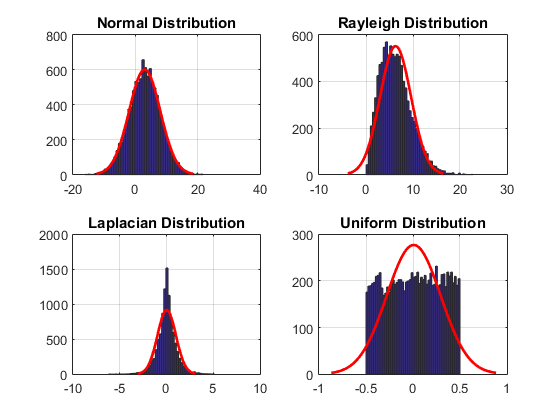
\includegraphics[width=\textwidth]{./22/hist.png}
		\caption[]{{\small Histogramas de las distribuciones.}}    
		\label{fig:22:histogram}
	\end{subfigure}
	\hfill
	\begin{subfigure}[b]{0.475 \textwidth}  
		\centering 
		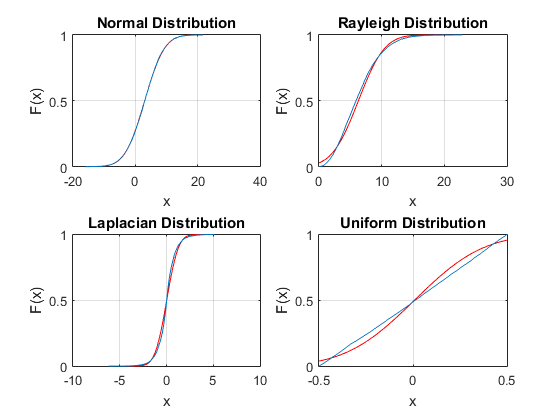
\includegraphics[width=\textwidth]{./22/cdfplot.png}
		\caption[]{{\small Funciones densidad de probabilidad de las distribuciones.}}    
		\label{fig:22:pdf}
	\end{subfigure}
	\vskip\baselineskip
	\begin{subfigure}[b]{0.475 \textwidth}   
		\centering 
		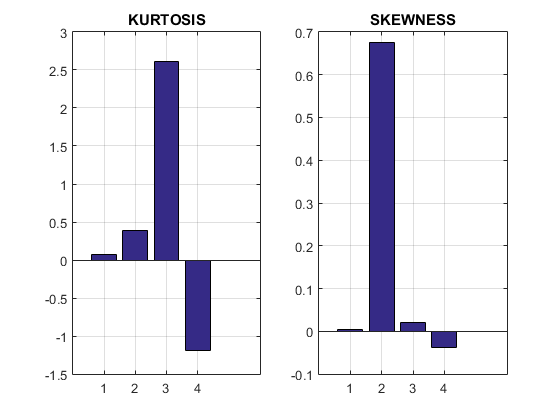
\includegraphics[width=\textwidth]{./22/kurtosis_skewness.png}
		\caption[]{{\small Gráficos de \emph{Skewness} y \emph{Kurtosis} de las distribuciones.}}    
		\label{fig:22:skew_kurt}
	\end{subfigure}
	\quad
	\begin{subfigure}[b]{0.475 \textwidth}   
		\centering 
		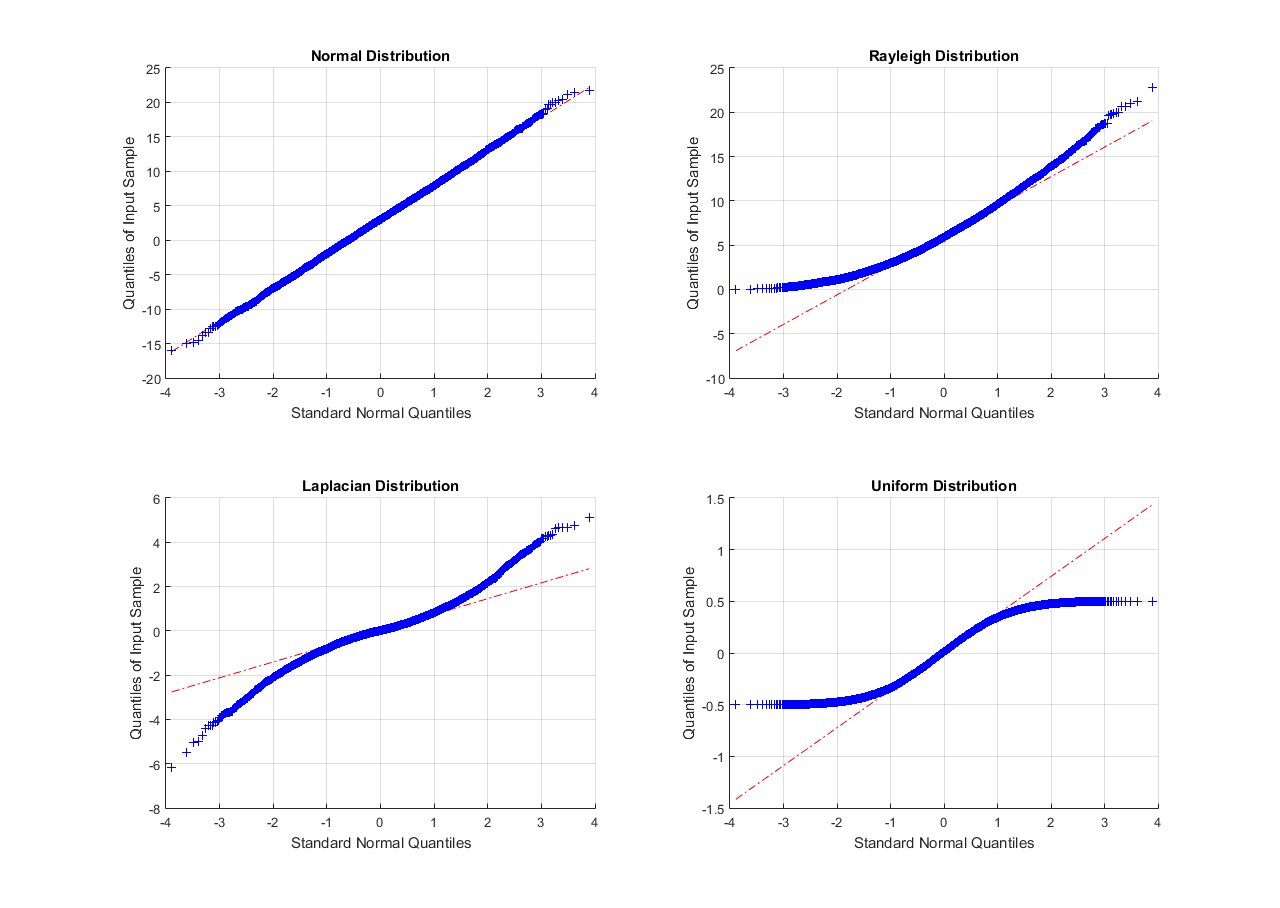
\includegraphics[width=\textwidth]{./22/normplot.png}
		\caption[]{{\small Gráficos \emph{NormPlot} de las distribuciones.}}    
		\label{fig:22:normplot}
	\end{subfigure}
	\caption[]{\small Gráficos de los tests de gausianidad de las cuatro distribuciones sintéticas.} 
	\label{fig:22:distributions}
\end{figure*}

\section{Observación de base de datos Brain}

Para los gráficos de esta sección se ha elegido mostrar las características de la clase \textbf{1 - Materia Gris}.

\subsection[Observaciones]{Observe y comente todas las gráficas obtenidas}

En la figura \ref{fig:23:gray} se pueden ver los gráficos para materia gris.

En la figura \ref{fig:23:gray:skew_kurt} se puede ver que las características 2 y 5 son las que tienen un \emph{Skewness} y \emph{Kurtosis} más parecidos a una distribución gausiana

En el \emph{Scatter plot} de la figura \ref{fig:23:gray:scatter} se ve como los pares de características 2 o 3 con 4 o 5 no son particularmente discriminativos.

En la figura \ref{fig:23:gray:cdf} vemos como el gráfico de CDF de la característica 1 es el que más se acerca al de una distribución gausiana.

Los histogramas de la figura \ref{fig:23:gray:hist} vemos como la característica 4 es la más parecida a una distribución gausiana, mientras que el resto de ellas muestran histogramas "picudos" o asimétricos.

Según los \emph{NormPlot} de la figura \ref{fig:23:gray:normplot}, la característica 2 está más cercana a ser gausiana, ya que el resto muestran severas diferencias respecto la recta de referencia.

\begin{figure*}[h]
	\centering
	\begin{subfigure}[b]{0.475 \textwidth}
		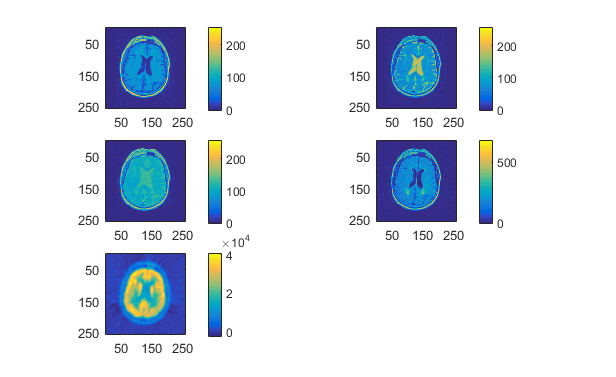
\includegraphics[width = \textwidth]{./23/caract.png}
		\caption{Representación en escala de colores de las características de la base de datos.}
		\label{fig:23:gray:caract}
	\end{subfigure}
	~
	\begin{subfigure}[b]{0.475 \textwidth}
		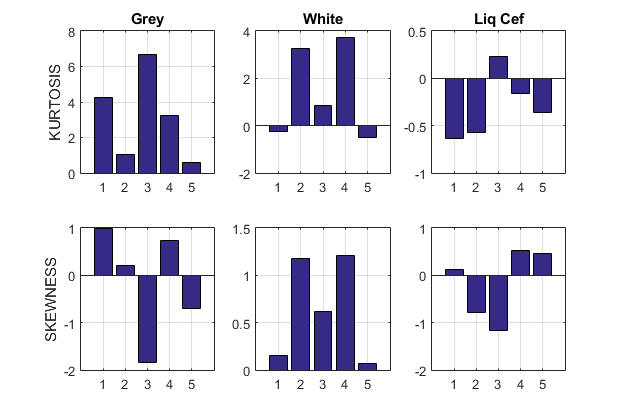
\includegraphics[width = \textwidth]{./23/kurtosis_skewness.png}
		\caption{Gráficos de \emph{Skewness} y \emph{Kurtosis}.}
		\label{fig:23:gray:skew_kurt}
	\end{subfigure}
	\vskip\baselineskip
	\begin{subfigure}[b]{0.475 \textwidth}
		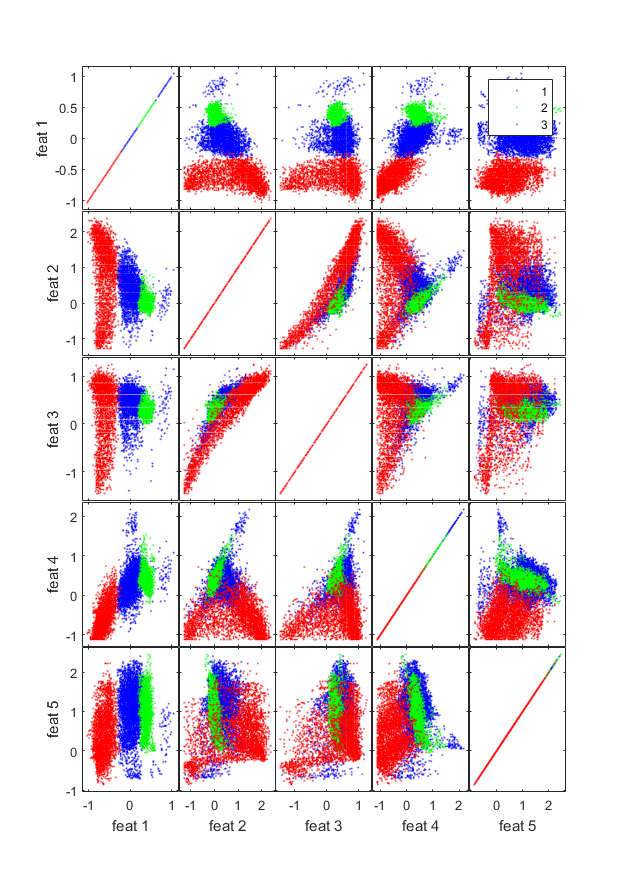
\includegraphics[width = \textwidth]{./23/scatter.png}
		\caption{\emph{Scatter plots} de todas las características.}
		\label{fig:23:gray:scatter}
	\end{subfigure}
	~
	\begin{subfigure}[b]{0.475 \textwidth}
		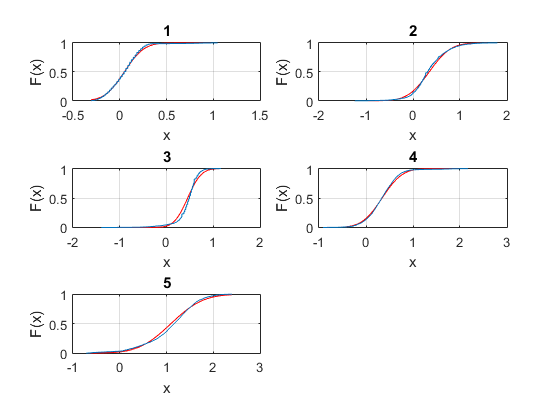
\includegraphics[width = \textwidth]{./23/1_gris/cdfplot.png}
		\caption{Histogramas acumulados para materia gris}
		\label{fig:23:gray:cdf}
	\end{subfigure}
	\vskip\baselineskip
	\begin{subfigure}[b]{0.475 \textwidth}
		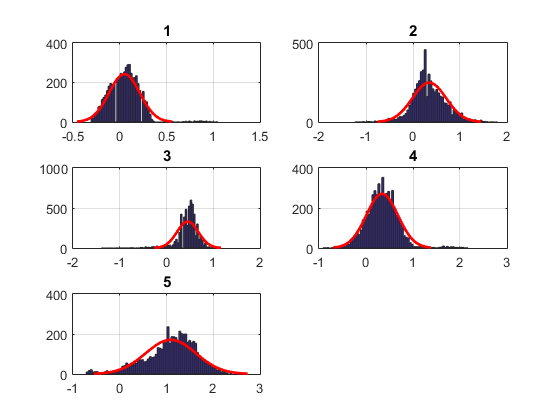
\includegraphics[width = \textwidth]{./23/1_gris/hist.png}
		\caption{Histogramas para materia gris}
		\label{fig:23:gray:hist}
	\end{subfigure}
	~
	\begin{subfigure}[b]{0.475 \textwidth}
		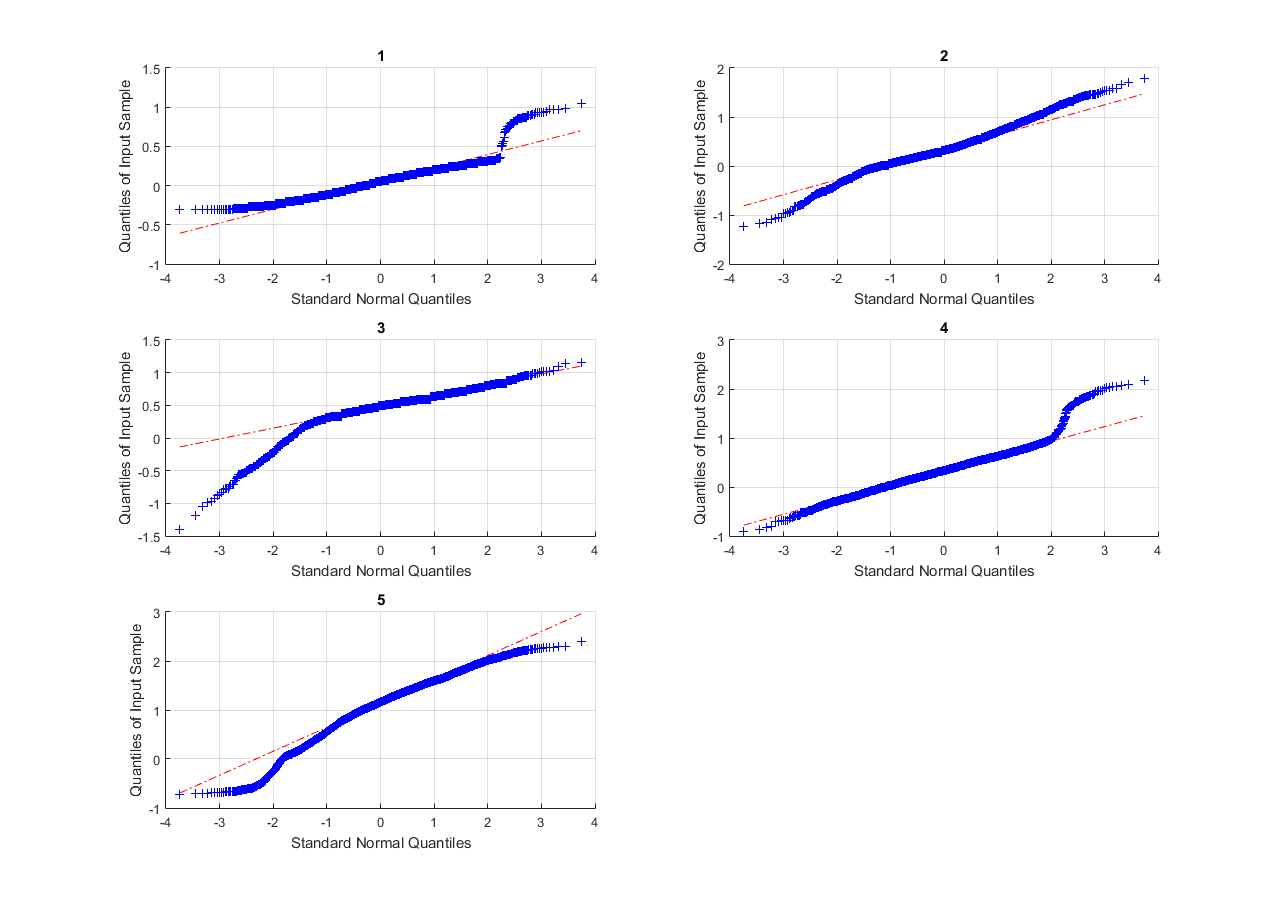
\includegraphics[width = \textwidth]{./23/1_gris/plotnorm.png}
		\caption{Gráficos \emph{NormPlot} para materia gris}
		\label{fig:23:gray:normplot}
	\end{subfigure}
	\caption{Gráficos de las mediciones sobre las características de materia gris.}
	\label{fig:23:gray}
\end{figure*}

\subsection[Subconjuntos]{A partir de la observación del “scatter plot”, proponga el subconjunto de 2 características o coordenadas que resulte más discriminativo para este caso}

En el \emph{Scatter Plot} de la figura \ref{fig:23:gray:scatter} se ve como la característica 1 es la que más separabilidad proporciona, especialmente con la característica 4.

Esta pareja de características concentra los puntos del gráfico de una forma más separada y compacta que el resto de combinaciones.

\subsection[Cambiar clases]{Cambie la clase analizada en la última parte del programa y copie los resultados obtenidos en el documento de resultados}

Las figuras \ref{fig:23:white} y \ref{fig:23:liquid} muestran los conjuntos de gráficos obtenidos para las dos clases restantes, \textbf{2 - Materia blanca} y \textbf{3 - Líquido cefaloraquídeo}, respectivamente.

\begin{figure*}[h]
	\centering
	\begin{subfigure}[b]{0.475 \textwidth}
		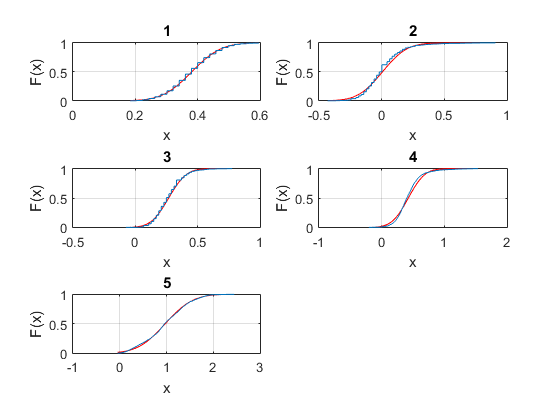
\includegraphics[width = \textwidth]{./23/2_blanca/cdfplot.png}
		\caption{Histogramas acumulados para materia blanca}
		\label{fig:23:white:cdf}
	\end{subfigure}
	~
	\begin{subfigure}[b]{0.475 \textwidth}
		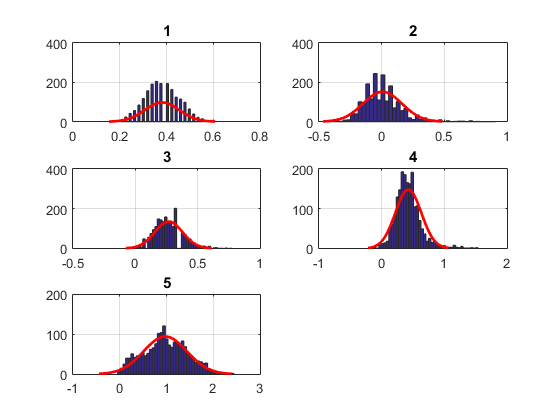
\includegraphics[width = \textwidth]{./23/2_blanca/hist.png}
		\caption{Histogramas para materia blanca}
		\label{fig:23:white:hist}
	\end{subfigure}
	\vskip\baselineskip
	\begin{subfigure}[b]{0.475 \textwidth}
		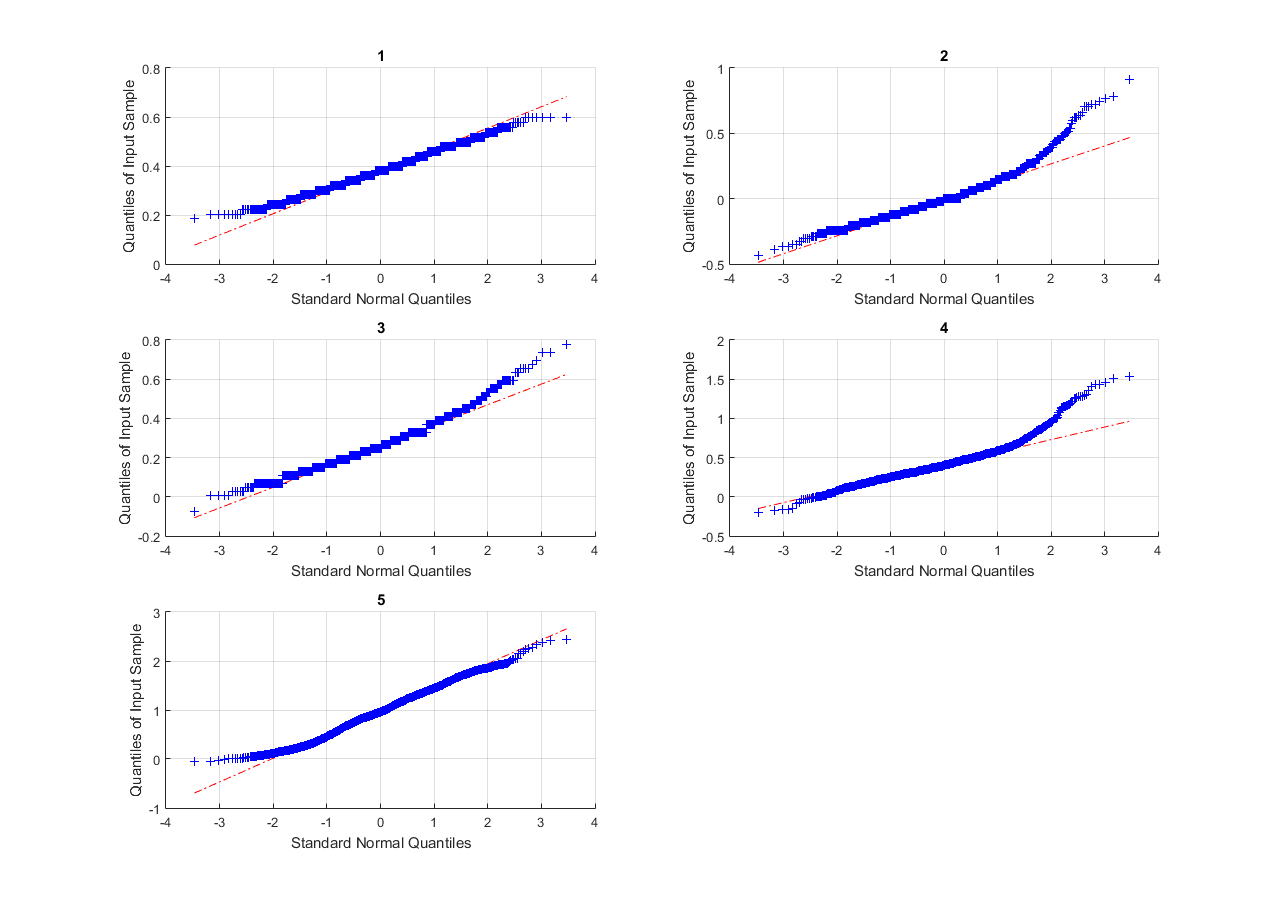
\includegraphics[width = \textwidth]{./23/2_blanca/plotnorm.png}
		\caption{Gráficos \emph{NormPlot} para materia blanca}
		\label{fig:23:white:normplot}
	\end{subfigure}
	\caption{Gráficos de las mediciones sobre las características de materia blanca.}
	\label{fig:23:white}
\end{figure*}

\begin{figure*}[h]
	\centering
	\begin{subfigure}[b]{0.475 \textwidth}
		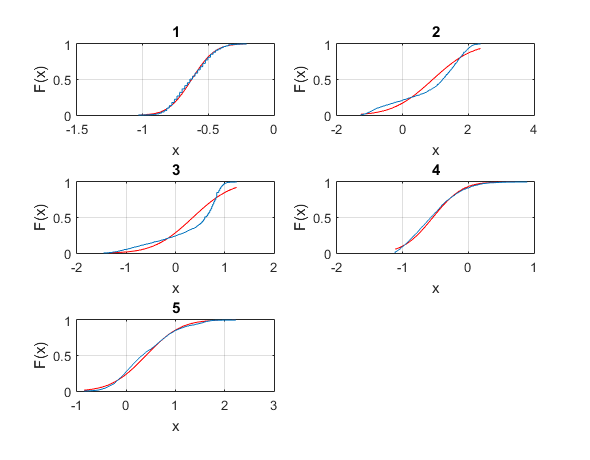
\includegraphics[width = \textwidth]{./23/3_liquido/cdfplot.png}
		\caption{Histogramas acumulados para líquido cefaloraquídeo}
		\label{fig:23:liquid:cdf}
	\end{subfigure}
	~
	\begin{subfigure}[b]{0.475 \textwidth}
		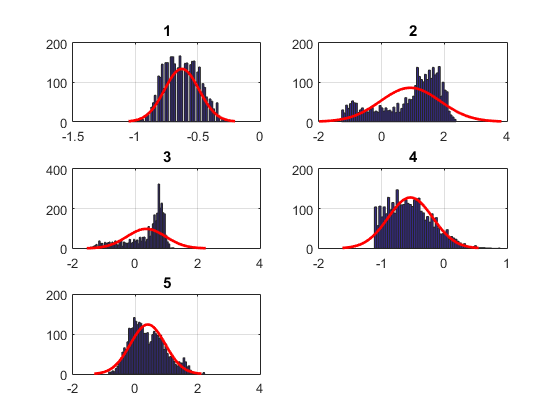
\includegraphics[width = \textwidth]{./23/3_liquido/hist.png}
		\caption{Histogramas para líquido cefaloraquídeo}
		\label{fig:23:liquid:hist}
	\end{subfigure}
	\vskip\baselineskip
	\begin{subfigure}[b]{0.475 \textwidth}
		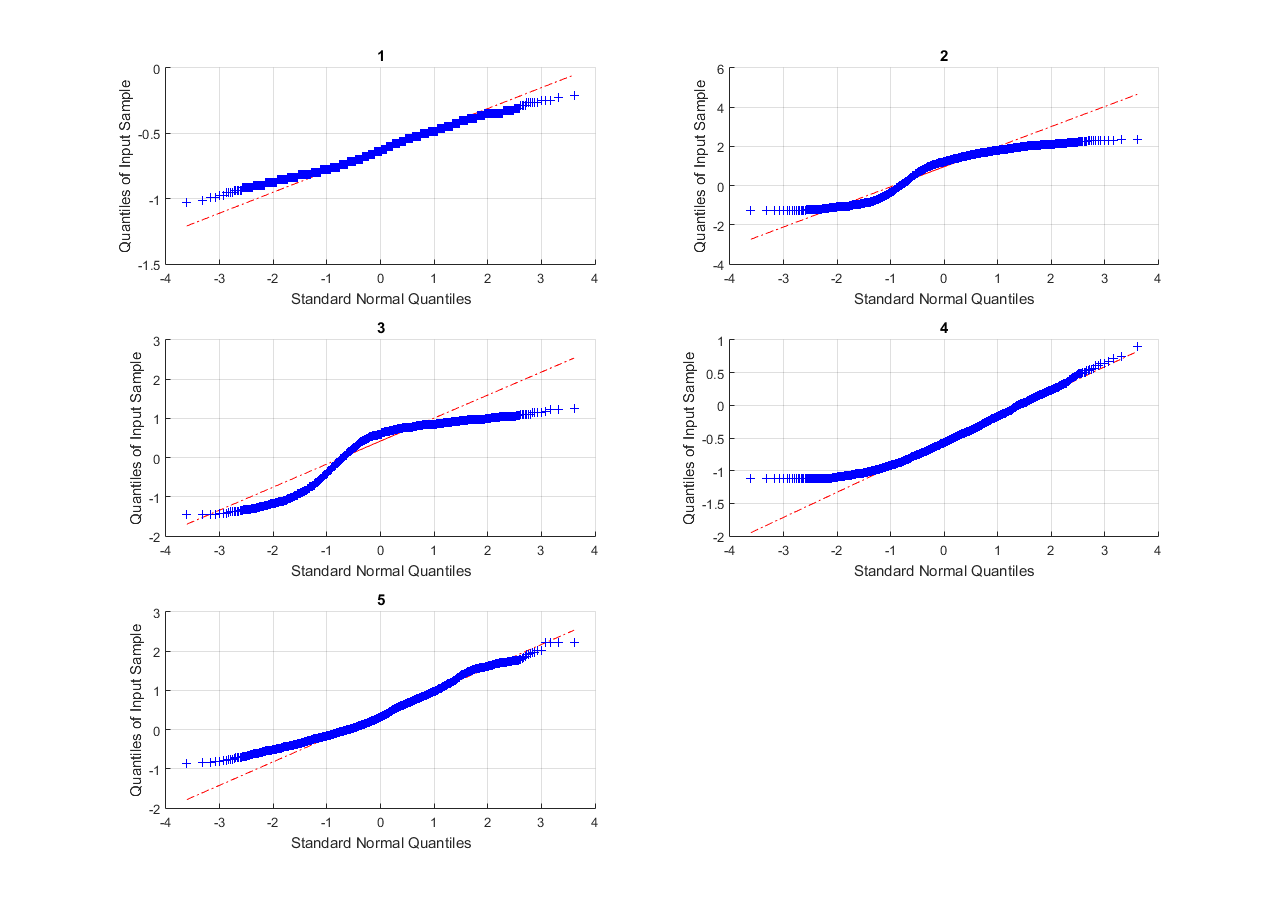
\includegraphics[width = \textwidth]{./23/3_liquido/plotnorm.png}
		\caption{Gráficos \emph{NormPlot} para líquido cefaloraquídeo}
		\label{fig:23:liquid:normplot}
	\end{subfigure}
	\caption{Gráficos de las mediciones sobre las características de líquido cefaloraquídeo.}
	\label{fig:23:liquid}
\end{figure*}

\end{document}
